\documentclass{standalone}
\usepackage{tikz}
\begin{document}

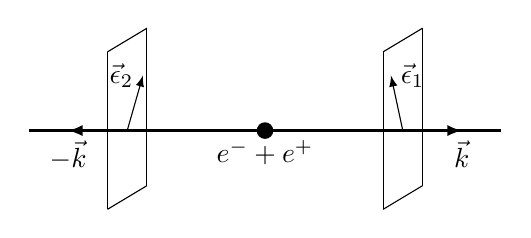
\begin{tikzpicture}
 \fill (0,0) circle (3pt);
 \node[below] at (0,0){$e^-+e^+$};
 \draw[latex-latex, thick] (-2.5,0)node[below]{$-\vec{k}$} --(2.5,0)node[below]{$\vec{k}$};
 \draw[thick] (-3,0) --(3,0);
 \draw[] (-2,-1)--(-2,1);
\draw[] (-1.5,-0.7)--(-1.5,1.3);
\draw (-2,1)--(-1.5,1.3);
\draw (-2,-1)--(-1.5,-0.7);
\draw[-latex] (-1.75,0)--(-1.55,0.7) node[left]{$\vec{\epsilon}_2$};;
\begin{scope}[shift={(3.5,0)}]
    \draw[] (-2,-1) -- (-2,1);
    \draw[] (-1.5,-0.7) -- (-1.5,1.3);
    \draw (-2,1) -- (-1.5,1.3);
    \draw (-2,-1) -- (-1.5,-0.7);
    \draw[-latex] (-1.75,0)--(-1.9,0.7)node[right]{$\vec{\epsilon}_1$};
\end{scope}


 
\end{tikzpicture}

\end{document}
